% !TeX root = ../../Report.tex
% !TeX encoding = UTF-8
در این قسمت تمام اطلاعات مربوط به کاربران ثبت می‌شود.

\begin{figure}[H]
	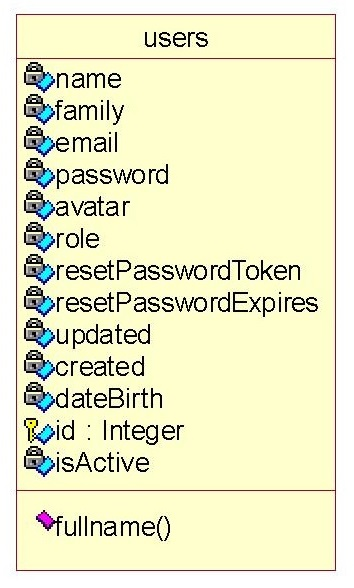
\includegraphics[width=.4\textwidth]{Diagram/6.Class/کاربر.jpg}
	\centering
	\caption{ساختار پایگاه داده کاربر}
	\label{fig:db:کاربر}
\end{figure}

\paragraph{\rl{name}:}
حاوی اطلاعات تام و نام‌خانوادگی.
\paragraph{\rl{username}:}
حاوی اطلاعات نام کاربری و تاریخچه تغییرات آن.
\paragraph{\rl{email}:}
حاوی اطلاعات پست الکترونیک و تاریخچه تغییرات آن.
\paragraph{\rl{password}:}
حاوی اطلاعات رمز عبور و تاریخچه تغییرات آن.
\paragraph{\rl{isActive}:}
 دسترسی کاربر به داشبورد‌ها را مشخص می‌کند.
\paragraph{\rl{avatar}:}
حاوی اطلاعات تصویر پروفایل کاربر.
\paragraph{\rl{role}:}
سطح دسترسی کاربر را مشخص می‌کند.